\documentclass[a4paper,10pt]{report}
\usepackage[utf8]{inputenc}
\usepackage[T1]{fontenc}
\usepackage[french]{babel}
\usepackage{lmodern}
\usepackage{graphicx}
\usepackage[11pt]{extsizes}
\usepackage{titlesec}
\usepackage[toc,page]{appendix}
\usepackage{listings}
\usepackage{color}
\usepackage{sectsty}
\usepackage{url}
\usepackage{graphicx}
\usepackage{ulem}
\usepackage{lscape}
\usepackage{listings}
\usepackage{color}

\definecolor{dkgreen}{rgb}{0,0.4,0}
\definecolor{gray}{rgb}{0.5,0.5,0.5}
\definecolor{mauve}{rgb}{0.58,0,0.82}

\lstset
{
  showstringspaces=false,
  columns=flexible,
  basicstyle={\small\ttfamily},
  numbers=none,
  numberstyle=\tiny\color{gray},
  keywordstyle=\color{dkgreen},
  commentstyle=\color{blue},
  stringstyle=\color{mauve},
  breaklines=true,
  breakatwhitespace=true,
  tabsize=4,
  morekeywords={boolean, unsigned}
}



\begin{document}
\begin{titlepage}
\begin{center}

	~~~~~~~
\includegraphics[scale=0.7]{university.png}~~~~~~~~~

		\HRule \\[2cm]
		\textsc{Master informatique M2}\\
		\HRule \\[2cm]

		{ \huge \bfseries Conduite de projet : Rapport TD3 \\[0.4cm] }

		\HRule \\[2cm]

		\noindent
		\begin{minipage}{0.5\textwidth}
		\begin{flushleft} \large
		\emph{Par:}\\
		\smallbreak
		Amira \textsc{Touati}\\
		Raphael \textsc{Jorel}\\
		Tristan \textsc{ Campbell}
		\end{flushleft}
		\end{minipage}%


		\vfill
		{\large \today}
		\end{center}

	\end{titlepage}
	\newpage
\section*{Les tâches :}
	\begin{itemize}
        \item T1 : Coder la base de données
        \item T2 : Coder l'architecture REST
        \item T3 : Coder la couche client (la vue)
        \item T4 : Coder la couche client (le modèle, le contrôleur)
        \item T5 : Faire les tests d'accès HTTP à la base de donnèes
        \item T6 : Faire les tests E2E.
    \end{itemize}
	\section*{Diagramme de Pert :}
    \begin{figure}[!h]
        \centering
        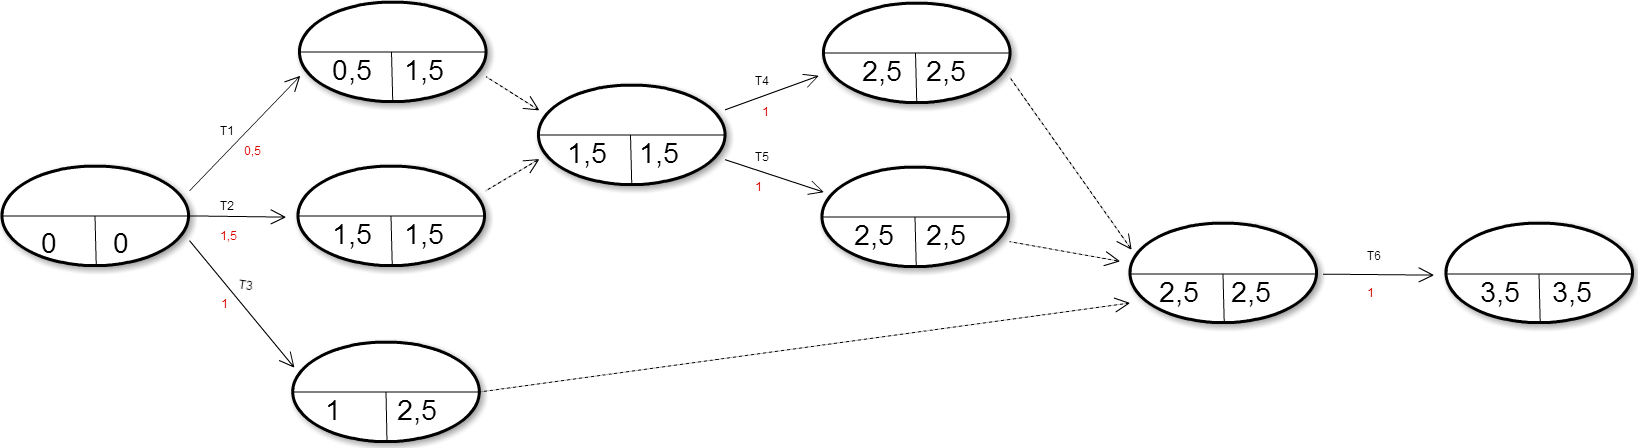
\includegraphics[scale=0.28]{plan.png}
        \caption[Diagramme de Pert]{Diagramme de Pert}
    \end{figure}


\section*{Diagramme de Gantt:}

\begin{tabular}{|l|c|c|c|c|c|c|r|}
  \hline
   & 0,5 & 1 & 1,5 & 2 & 2,5 & 3 & 3,5\\
  \hline
  Campbell &  &  &  & T3 & T3 & T5 & T5 \\
  Jorel & T2 & T2 & T2 & & &  &  \\
  Touati & T1 & T3 & T3 & T4 & T4 & & \\
  \hline
\end{tabular}

\newpage

\section*{Coder la base de données}
	\begin{figure}[!h]
    \centering
    %\includegraphics[scale=0.80]{BD.png}
    \lstinputlisting[language=sql]{table.sql}
    \caption[Base de données]{Base de données}
    \end{figure}

\end{document}
